\documentclass[11pt,reqno]{amsart}
\usepackage[T1]{fontenc}
\usepackage{amsmath}
\usepackage{amssymb}
\usepackage[colorlinks, citecolor = blue, linkcolor = blue]{hyperref}
\usepackage[dvipsnames]{xcolor}
\usepackage{tikz}
\usetikzlibrary{matrix}
\usetikzlibrary{patterns}
\usetikzlibrary{matrix}
\usetikzlibrary{positioning}
\usetikzlibrary{decorations.pathmorphing}
\usetikzlibrary{cd}
\usetikzlibrary{intersections,calc}
\tikzset{dot/.style={circle, fill=black, inner sep=.05cm}}

\begin{document}

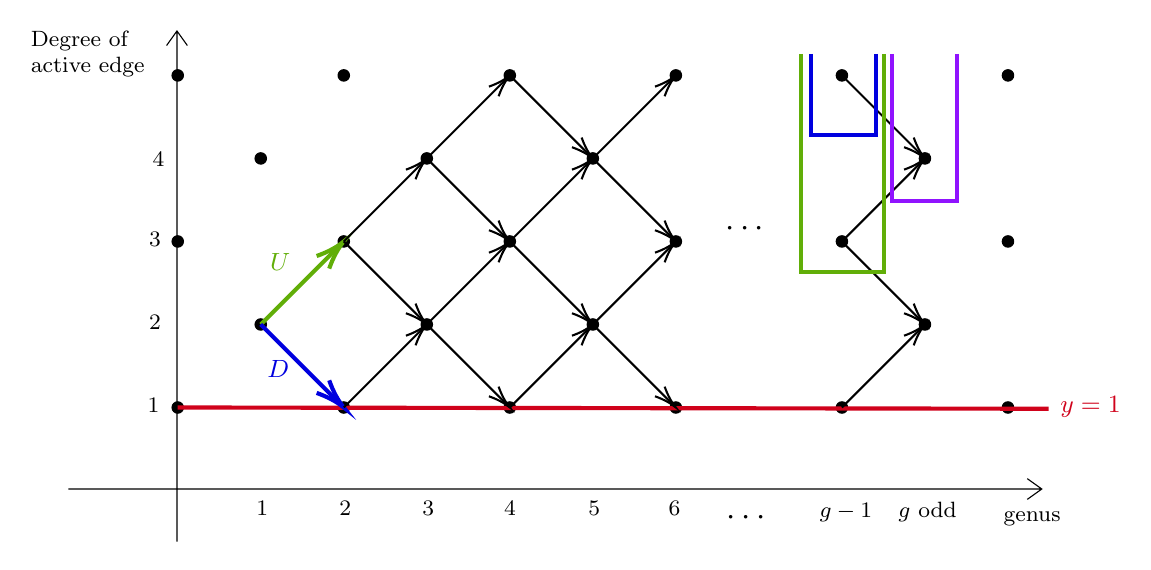
\begin{tikzpicture}[x=0.75pt,y=0.75pt,yscale=-1,xscale=1]

\draw  (48,249.67) -- (517,249.67)(100.33,29) -- (100.33,275) (510,244.67) -- (517,249.67) -- (510,254.67) (95.33,36) -- (100.33,29) -- (105.33,36)  ;
\draw   (100,161) .. controls (100,161) and (100,161) .. (100,161) .. controls (100,161) and (100,161) .. (100,161) .. controls (100,161) and (100,161) .. (100,161) .. controls (100,161) and (100,161) .. (100,161) -- cycle ;
\draw  [fill={rgb, 255:red, 0; green, 0; blue, 0 }  ,fill opacity=1 ] (97.95,130.4) .. controls (97.95,128.88) and (99.18,127.65) .. (100.7,127.65) .. controls (102.22,127.65) and (103.45,128.88) .. (103.45,130.4) .. controls (103.45,131.92) and (102.22,133.15) .. (100.7,133.15) .. controls (99.18,133.15) and (97.95,131.92) .. (97.95,130.4) -- cycle ;
\draw  [fill={rgb, 255:red, 0; green, 0; blue, 0 }  ,fill opacity=1 ] (97.95,210.4) .. controls (97.95,208.88) and (99.18,207.65) .. (100.7,207.65) .. controls (102.22,207.65) and (103.45,208.88) .. (103.45,210.4) .. controls (103.45,211.92) and (102.22,213.15) .. (100.7,213.15) .. controls (99.18,213.15) and (97.95,211.92) .. (97.95,210.4) -- cycle ;
\draw  [fill={rgb, 255:red, 0; green, 0; blue, 0 }  ,fill opacity=1 ] (137.95,170.4) .. controls (137.95,168.88) and (139.18,167.65) .. (140.7,167.65) .. controls (142.22,167.65) and (143.45,168.88) .. (143.45,170.4) .. controls (143.45,171.92) and (142.22,173.15) .. (140.7,173.15) .. controls (139.18,173.15) and (137.95,171.92) .. (137.95,170.4) -- cycle ;
\draw  [fill={rgb, 255:red, 0; green, 0; blue, 0 }  ,fill opacity=1 ] (177.95,210.4) .. controls (177.95,208.88) and (179.18,207.65) .. (180.7,207.65) .. controls (182.22,207.65) and (183.45,208.88) .. (183.45,210.4) .. controls (183.45,211.92) and (182.22,213.15) .. (180.7,213.15) .. controls (179.18,213.15) and (177.95,211.92) .. (177.95,210.4) -- cycle ;
\draw  [fill={rgb, 255:red, 0; green, 0; blue, 0 }  ,fill opacity=1 ] (177.95,130.4) .. controls (177.95,128.88) and (179.18,127.65) .. (180.7,127.65) .. controls (182.22,127.65) and (183.45,128.88) .. (183.45,130.4) .. controls (183.45,131.92) and (182.22,133.15) .. (180.7,133.15) .. controls (179.18,133.15) and (177.95,131.92) .. (177.95,130.4) -- cycle ;
\draw  [fill={rgb, 255:red, 0; green, 0; blue, 0 }  ,fill opacity=1 ] (217.95,170.4) .. controls (217.95,168.88) and (219.18,167.65) .. (220.7,167.65) .. controls (222.22,167.65) and (223.45,168.88) .. (223.45,170.4) .. controls (223.45,171.92) and (222.22,173.15) .. (220.7,173.15) .. controls (219.18,173.15) and (217.95,171.92) .. (217.95,170.4) -- cycle ;
\draw  [fill={rgb, 255:red, 0; green, 0; blue, 0 }  ,fill opacity=1 ] (137.95,90.4) .. controls (137.95,88.88) and (139.18,87.65) .. (140.7,87.65) .. controls (142.22,87.65) and (143.45,88.88) .. (143.45,90.4) .. controls (143.45,91.92) and (142.22,93.15) .. (140.7,93.15) .. controls (139.18,93.15) and (137.95,91.92) .. (137.95,90.4) -- cycle ;
\draw  [fill={rgb, 255:red, 0; green, 0; blue, 0 }  ,fill opacity=1 ] (217.95,90.4) .. controls (217.95,88.88) and (219.18,87.65) .. (220.7,87.65) .. controls (222.22,87.65) and (223.45,88.88) .. (223.45,90.4) .. controls (223.45,91.92) and (222.22,93.15) .. (220.7,93.15) .. controls (219.18,93.15) and (217.95,91.92) .. (217.95,90.4) -- cycle ;
\draw  [fill={rgb, 255:red, 0; green, 0; blue, 0 }  ,fill opacity=1 ] (97.95,50.4) .. controls (97.95,48.88) and (99.18,47.65) .. (100.7,47.65) .. controls (102.22,47.65) and (103.45,48.88) .. (103.45,50.4) .. controls (103.45,51.92) and (102.22,53.15) .. (100.7,53.15) .. controls (99.18,53.15) and (97.95,51.92) .. (97.95,50.4) -- cycle ;
\draw  [fill={rgb, 255:red, 0; green, 0; blue, 0 }  ,fill opacity=1 ] (177.95,50.4) .. controls (177.95,48.88) and (179.18,47.65) .. (180.7,47.65) .. controls (182.22,47.65) and (183.45,48.88) .. (183.45,50.4) .. controls (183.45,51.92) and (182.22,53.15) .. (180.7,53.15) .. controls (179.18,53.15) and (177.95,51.92) .. (177.95,50.4) -- cycle ;
\draw  [fill={rgb, 255:red, 0; green, 0; blue, 0 }  ,fill opacity=1 ] (257.95,50.4) .. controls (257.95,48.88) and (259.18,47.65) .. (260.7,47.65) .. controls (262.22,47.65) and (263.45,48.88) .. (263.45,50.4) .. controls (263.45,51.92) and (262.22,53.15) .. (260.7,53.15) .. controls (259.18,53.15) and (257.95,51.92) .. (257.95,50.4) -- cycle ;
\draw  [fill={rgb, 255:red, 0; green, 0; blue, 0 }  ,fill opacity=1 ] (257.95,130.4) .. controls (257.95,128.88) and (259.18,127.65) .. (260.7,127.65) .. controls (262.22,127.65) and (263.45,128.88) .. (263.45,130.4) .. controls (263.45,131.92) and (262.22,133.15) .. (260.7,133.15) .. controls (259.18,133.15) and (257.95,131.92) .. (257.95,130.4) -- cycle ;
\draw  [fill={rgb, 255:red, 0; green, 0; blue, 0 }  ,fill opacity=1 ] (257.95,210.4) .. controls (257.95,208.88) and (259.18,207.65) .. (260.7,207.65) .. controls (262.22,207.65) and (263.45,208.88) .. (263.45,210.4) .. controls (263.45,211.92) and (262.22,213.15) .. (260.7,213.15) .. controls (259.18,213.15) and (257.95,211.92) .. (257.95,210.4) -- cycle ;
\draw  [fill={rgb, 255:red, 0; green, 0; blue, 0 }  ,fill opacity=1 ] (297.95,170.4) .. controls (297.95,168.88) and (299.18,167.65) .. (300.7,167.65) .. controls (302.22,167.65) and (303.45,168.88) .. (303.45,170.4) .. controls (303.45,171.92) and (302.22,173.15) .. (300.7,173.15) .. controls (299.18,173.15) and (297.95,171.92) .. (297.95,170.4) -- cycle ;
\draw  [fill={rgb, 255:red, 0; green, 0; blue, 0 }  ,fill opacity=1 ] (337.95,210.4) .. controls (337.95,208.88) and (339.18,207.65) .. (340.7,207.65) .. controls (342.22,207.65) and (343.45,208.88) .. (343.45,210.4) .. controls (343.45,211.92) and (342.22,213.15) .. (340.7,213.15) .. controls (339.18,213.15) and (337.95,211.92) .. (337.95,210.4) -- cycle ;
\draw  [fill={rgb, 255:red, 0; green, 0; blue, 0 }  ,fill opacity=1 ] (337.95,130.4) .. controls (337.95,128.88) and (339.18,127.65) .. (340.7,127.65) .. controls (342.22,127.65) and (343.45,128.88) .. (343.45,130.4) .. controls (343.45,131.92) and (342.22,133.15) .. (340.7,133.15) .. controls (339.18,133.15) and (337.95,131.92) .. (337.95,130.4) -- cycle ;
\draw  [fill={rgb, 255:red, 0; green, 0; blue, 0 }  ,fill opacity=1 ] (417.95,210.4) .. controls (417.95,208.88) and (419.18,207.65) .. (420.7,207.65) .. controls (422.22,207.65) and (423.45,208.88) .. (423.45,210.4) .. controls (423.45,211.92) and (422.22,213.15) .. (420.7,213.15) .. controls (419.18,213.15) and (417.95,211.92) .. (417.95,210.4) -- cycle ;
\draw  [fill={rgb, 255:red, 0; green, 0; blue, 0 }  ,fill opacity=1 ] (417.95,130.4) .. controls (417.95,128.88) and (419.18,127.65) .. (420.7,127.65) .. controls (422.22,127.65) and (423.45,128.88) .. (423.45,130.4) .. controls (423.45,131.92) and (422.22,133.15) .. (420.7,133.15) .. controls (419.18,133.15) and (417.95,131.92) .. (417.95,130.4) -- cycle ;
\draw  [fill={rgb, 255:red, 0; green, 0; blue, 0 }  ,fill opacity=1 ] (457.95,170.4) .. controls (457.95,168.88) and (459.18,167.65) .. (460.7,167.65) .. controls (462.22,167.65) and (463.45,168.88) .. (463.45,170.4) .. controls (463.45,171.92) and (462.22,173.15) .. (460.7,173.15) .. controls (459.18,173.15) and (457.95,171.92) .. (457.95,170.4) -- cycle ;
\draw  [fill={rgb, 255:red, 0; green, 0; blue, 0 }  ,fill opacity=1 ] (497.95,210.4) .. controls (497.95,208.88) and (499.18,207.65) .. (500.7,207.65) .. controls (502.22,207.65) and (503.45,208.88) .. (503.45,210.4) .. controls (503.45,211.92) and (502.22,213.15) .. (500.7,213.15) .. controls (499.18,213.15) and (497.95,211.92) .. (497.95,210.4) -- cycle ;
\draw  [fill={rgb, 255:red, 0; green, 0; blue, 0 }  ,fill opacity=1 ] (497.95,130.4) .. controls (497.95,128.88) and (499.18,127.65) .. (500.7,127.65) .. controls (502.22,127.65) and (503.45,128.88) .. (503.45,130.4) .. controls (503.45,131.92) and (502.22,133.15) .. (500.7,133.15) .. controls (499.18,133.15) and (497.95,131.92) .. (497.95,130.4) -- cycle ;
\draw  [fill={rgb, 255:red, 0; green, 0; blue, 0 }  ,fill opacity=1 ] (297.95,90.4) .. controls (297.95,88.88) and (299.18,87.65) .. (300.7,87.65) .. controls (302.22,87.65) and (303.45,88.88) .. (303.45,90.4) .. controls (303.45,91.92) and (302.22,93.15) .. (300.7,93.15) .. controls (299.18,93.15) and (297.95,91.92) .. (297.95,90.4) -- cycle ;
\draw  [fill={rgb, 255:red, 0; green, 0; blue, 0 }  ,fill opacity=1 ] (337.95,50.4) .. controls (337.95,48.88) and (339.18,47.65) .. (340.7,47.65) .. controls (342.22,47.65) and (343.45,48.88) .. (343.45,50.4) .. controls (343.45,51.92) and (342.22,53.15) .. (340.7,53.15) .. controls (339.18,53.15) and (337.95,51.92) .. (337.95,50.4) -- cycle ;
\draw  [fill={rgb, 255:red, 0; green, 0; blue, 0 }  ,fill opacity=1 ] (417.95,50.4) .. controls (417.95,48.88) and (419.18,47.65) .. (420.7,47.65) .. controls (422.22,47.65) and (423.45,48.88) .. (423.45,50.4) .. controls (423.45,51.92) and (422.22,53.15) .. (420.7,53.15) .. controls (419.18,53.15) and (417.95,51.92) .. (417.95,50.4) -- cycle ;
\draw  [fill={rgb, 255:red, 0; green, 0; blue, 0 }  ,fill opacity=1 ] (457.95,90.4) .. controls (457.95,88.88) and (459.18,87.65) .. (460.7,87.65) .. controls (462.22,87.65) and (463.45,88.88) .. (463.45,90.4) .. controls (463.45,91.92) and (462.22,93.15) .. (460.7,93.15) .. controls (459.18,93.15) and (457.95,91.92) .. (457.95,90.4) -- cycle ;
\draw  [fill={rgb, 255:red, 0; green, 0; blue, 0 }  ,fill opacity=1 ] (497.95,50.4) .. controls (497.95,48.88) and (499.18,47.65) .. (500.7,47.65) .. controls (502.22,47.65) and (503.45,48.88) .. (503.45,50.4) .. controls (503.45,51.92) and (502.22,53.15) .. (500.7,53.15) .. controls (499.18,53.15) and (497.95,51.92) .. (497.95,50.4) -- cycle ;
\draw [color={rgb, 255:red, 208; green, 2; blue, 27 }  ,draw opacity=1 ][line width=1.5]    (100.7,210.4) -- (520.33,211) ;
\draw [color={rgb, 255:red, 97; green, 174; blue, 8 }  ,draw opacity=1 ][line width=1.5]    (140.7,170.4) -- (178.58,132.52) ;
\draw [shift={(180.7,130.4)}, rotate = 135] [color={rgb, 255:red, 97; green, 174; blue, 8 }  ,draw opacity=1 ][line width=1.5]    (14.21,-4.28) .. controls (9.04,-1.82) and (4.3,-0.39) .. (0,0) .. controls (4.3,0.39) and (9.04,1.82) .. (14.21,4.28)   ;
\draw [color={rgb, 255:red, 0; green, 0; blue, 223 }  ,draw opacity=1 ][line width=1.5]    (140.7,170.4) -- (178.58,208.28) ;
\draw [shift={(180.7,210.4)}, rotate = 225] [color={rgb, 255:red, 0; green, 0; blue, 223 }  ,draw opacity=1 ][line width=1.5]    (14.21,-4.28) .. controls (9.04,-1.82) and (4.3,-0.39) .. (0,0) .. controls (4.3,0.39) and (9.04,1.82) .. (14.21,4.28)   ;
\draw [color={rgb, 255:red, 0; green, 0; blue, 0 }  ,draw opacity=1 ][line width=0.75]    (180.7,210.4) -- (219.29,171.81) ;
\draw [shift={(220.7,170.4)}, rotate = 135] [color={rgb, 255:red, 0; green, 0; blue, 0 }  ,draw opacity=1 ][line width=0.75]    (10.93,-3.29) .. controls (6.95,-1.4) and (3.31,-0.3) .. (0,0) .. controls (3.31,0.3) and (6.95,1.4) .. (10.93,3.29)   ;
\draw [color={rgb, 255:red, 0; green, 0; blue, 0 }  ,draw opacity=1 ][line width=0.75]    (220.7,170.4) -- (259.29,131.81) ;
\draw [shift={(260.7,130.4)}, rotate = 135] [color={rgb, 255:red, 0; green, 0; blue, 0 }  ,draw opacity=1 ][line width=0.75]    (10.93,-3.29) .. controls (6.95,-1.4) and (3.31,-0.3) .. (0,0) .. controls (3.31,0.3) and (6.95,1.4) .. (10.93,3.29)   ;
\draw [color={rgb, 255:red, 0; green, 0; blue, 0 }  ,draw opacity=1 ][line width=0.75]    (180.7,130.4) -- (219.29,91.81) ;
\draw [shift={(220.7,90.4)}, rotate = 135] [color={rgb, 255:red, 0; green, 0; blue, 0 }  ,draw opacity=1 ][line width=0.75]    (10.93,-3.29) .. controls (6.95,-1.4) and (3.31,-0.3) .. (0,0) .. controls (3.31,0.3) and (6.95,1.4) .. (10.93,3.29)   ;
\draw [color={rgb, 255:red, 0; green, 0; blue, 0 }  ,draw opacity=1 ][line width=0.75]    (220.7,90.4) -- (259.29,51.81) ;
\draw [shift={(260.7,50.4)}, rotate = 135] [color={rgb, 255:red, 0; green, 0; blue, 0 }  ,draw opacity=1 ][line width=0.75]    (10.93,-3.29) .. controls (6.95,-1.4) and (3.31,-0.3) .. (0,0) .. controls (3.31,0.3) and (6.95,1.4) .. (10.93,3.29)   ;
\draw [color={rgb, 255:red, 0; green, 0; blue, 0 }  ,draw opacity=1 ][line width=0.75]    (260.7,210.4) -- (299.29,171.81) ;
\draw [shift={(300.7,170.4)}, rotate = 135] [color={rgb, 255:red, 0; green, 0; blue, 0 }  ,draw opacity=1 ][line width=0.75]    (10.93,-3.29) .. controls (6.95,-1.4) and (3.31,-0.3) .. (0,0) .. controls (3.31,0.3) and (6.95,1.4) .. (10.93,3.29)   ;
\draw [color={rgb, 255:red, 0; green, 0; blue, 0 }  ,draw opacity=1 ][line width=0.75]    (260.7,130.4) -- (299.29,91.81) ;
\draw [shift={(300.7,90.4)}, rotate = 135] [color={rgb, 255:red, 0; green, 0; blue, 0 }  ,draw opacity=1 ][line width=0.75]    (10.93,-3.29) .. controls (6.95,-1.4) and (3.31,-0.3) .. (0,0) .. controls (3.31,0.3) and (6.95,1.4) .. (10.93,3.29)   ;
\draw [color={rgb, 255:red, 0; green, 0; blue, 0 }  ,draw opacity=1 ][line width=0.75]    (300.7,170.4) -- (339.29,131.81) ;
\draw [shift={(340.7,130.4)}, rotate = 135] [color={rgb, 255:red, 0; green, 0; blue, 0 }  ,draw opacity=1 ][line width=0.75]    (10.93,-3.29) .. controls (6.95,-1.4) and (3.31,-0.3) .. (0,0) .. controls (3.31,0.3) and (6.95,1.4) .. (10.93,3.29)   ;
\draw [color={rgb, 255:red, 0; green, 0; blue, 0 }  ,draw opacity=1 ][line width=0.75]    (300.7,90.4) -- (339.29,51.81) ;
\draw [shift={(340.7,50.4)}, rotate = 135] [color={rgb, 255:red, 0; green, 0; blue, 0 }  ,draw opacity=1 ][line width=0.75]    (10.93,-3.29) .. controls (6.95,-1.4) and (3.31,-0.3) .. (0,0) .. controls (3.31,0.3) and (6.95,1.4) .. (10.93,3.29)   ;
\draw [color={rgb, 255:red, 0; green, 0; blue, 0 }  ,draw opacity=1 ][line width=0.75]    (180.7,130.4) -- (219.29,168.99) ;
\draw [shift={(220.7,170.4)}, rotate = 225] [color={rgb, 255:red, 0; green, 0; blue, 0 }  ,draw opacity=1 ][line width=0.75]    (10.93,-3.29) .. controls (6.95,-1.4) and (3.31,-0.3) .. (0,0) .. controls (3.31,0.3) and (6.95,1.4) .. (10.93,3.29)   ;
\draw [color={rgb, 255:red, 0; green, 0; blue, 0 }  ,draw opacity=1 ][line width=0.75]    (220.7,90.4) -- (259.29,128.99) ;
\draw [shift={(260.7,130.4)}, rotate = 225] [color={rgb, 255:red, 0; green, 0; blue, 0 }  ,draw opacity=1 ][line width=0.75]    (10.93,-3.29) .. controls (6.95,-1.4) and (3.31,-0.3) .. (0,0) .. controls (3.31,0.3) and (6.95,1.4) .. (10.93,3.29)   ;
\draw [color={rgb, 255:red, 0; green, 0; blue, 0 }  ,draw opacity=1 ][line width=0.75]    (220.7,170.4) -- (259.29,208.99) ;
\draw [shift={(260.7,210.4)}, rotate = 225] [color={rgb, 255:red, 0; green, 0; blue, 0 }  ,draw opacity=1 ][line width=0.75]    (10.93,-3.29) .. controls (6.95,-1.4) and (3.31,-0.3) .. (0,0) .. controls (3.31,0.3) and (6.95,1.4) .. (10.93,3.29)   ;
\draw [color={rgb, 255:red, 0; green, 0; blue, 0 }  ,draw opacity=1 ][line width=0.75]    (260.7,130.4) -- (299.29,168.99) ;
\draw [shift={(300.7,170.4)}, rotate = 225] [color={rgb, 255:red, 0; green, 0; blue, 0 }  ,draw opacity=1 ][line width=0.75]    (10.93,-3.29) .. controls (6.95,-1.4) and (3.31,-0.3) .. (0,0) .. controls (3.31,0.3) and (6.95,1.4) .. (10.93,3.29)   ;
\draw [color={rgb, 255:red, 0; green, 0; blue, 0 }  ,draw opacity=1 ][line width=0.75]    (300.7,90.4) -- (339.29,128.99) ;
\draw [shift={(340.7,130.4)}, rotate = 225] [color={rgb, 255:red, 0; green, 0; blue, 0 }  ,draw opacity=1 ][line width=0.75]    (10.93,-3.29) .. controls (6.95,-1.4) and (3.31,-0.3) .. (0,0) .. controls (3.31,0.3) and (6.95,1.4) .. (10.93,3.29)   ;
\draw [color={rgb, 255:red, 0; green, 0; blue, 0 }  ,draw opacity=1 ][line width=0.75]    (260.7,50.4) -- (299.29,88.99) ;
\draw [shift={(300.7,90.4)}, rotate = 225] [color={rgb, 255:red, 0; green, 0; blue, 0 }  ,draw opacity=1 ][line width=0.75]    (10.93,-3.29) .. controls (6.95,-1.4) and (3.31,-0.3) .. (0,0) .. controls (3.31,0.3) and (6.95,1.4) .. (10.93,3.29)   ;
\draw [color={rgb, 255:red, 0; green, 0; blue, 0 }  ,draw opacity=1 ][line width=0.75]    (300.7,170.4) -- (339.29,208.99) ;
\draw [shift={(340.7,210.4)}, rotate = 225] [color={rgb, 255:red, 0; green, 0; blue, 0 }  ,draw opacity=1 ][line width=0.75]    (10.93,-3.29) .. controls (6.95,-1.4) and (3.31,-0.3) .. (0,0) .. controls (3.31,0.3) and (6.95,1.4) .. (10.93,3.29)   ;
\draw [color={rgb, 255:red, 0; green, 0; blue, 0 }  ,draw opacity=1 ][line width=0.75]    (420.7,50.4) -- (459.29,88.99) ;
\draw [shift={(460.7,90.4)}, rotate = 225] [color={rgb, 255:red, 0; green, 0; blue, 0 }  ,draw opacity=1 ][line width=0.75]    (10.93,-3.29) .. controls (6.95,-1.4) and (3.31,-0.3) .. (0,0) .. controls (3.31,0.3) and (6.95,1.4) .. (10.93,3.29)   ;
\draw [color={rgb, 255:red, 0; green, 0; blue, 0 }  ,draw opacity=1 ][line width=0.75]    (420.7,130.4) -- (459.29,168.99) ;
\draw [shift={(460.7,170.4)}, rotate = 225] [color={rgb, 255:red, 0; green, 0; blue, 0 }  ,draw opacity=1 ][line width=0.75]    (10.93,-3.29) .. controls (6.95,-1.4) and (3.31,-0.3) .. (0,0) .. controls (3.31,0.3) and (6.95,1.4) .. (10.93,3.29)   ;
\draw [color={rgb, 255:red, 0; green, 0; blue, 0 }  ,draw opacity=1 ][line width=0.75]    (420.7,130.4) -- (459.29,91.81) ;
\draw [shift={(460.7,90.4)}, rotate = 135] [color={rgb, 255:red, 0; green, 0; blue, 0 }  ,draw opacity=1 ][line width=0.75]    (10.93,-3.29) .. controls (6.95,-1.4) and (3.31,-0.3) .. (0,0) .. controls (3.31,0.3) and (6.95,1.4) .. (10.93,3.29)   ;
\draw [color={rgb, 255:red, 0; green, 0; blue, 0 }  ,draw opacity=1 ][line width=0.75]    (420.7,210.4) -- (459.29,171.81) ;
\draw [shift={(460.7,170.4)}, rotate = 135] [color={rgb, 255:red, 0; green, 0; blue, 0 }  ,draw opacity=1 ][line width=0.75]    (10.93,-3.29) .. controls (6.95,-1.4) and (3.31,-0.3) .. (0,0) .. controls (3.31,0.3) and (6.95,1.4) .. (10.93,3.29)   ;
\draw  [color={rgb, 255:red, 144; green, 19; blue, 254 }  ,draw opacity=1 ][line width=1.5]  (476,40) -- (476,111) -- (452,111) ;
\draw  [color={rgb, 255:red, 144; green, 19; blue, 254 }  ,draw opacity=1 ][line width=1.5]  (445,40) -- (445,111) -- (452,111) ;

\draw  [color={rgb, 255:red, 0; green, 0; blue, 223 }  ,draw opacity=1 ][line width=1.5]  (437,40) -- (437,79) -- (413,79) ;
\draw  [color={rgb, 255:red, 0; green, 0; blue, 223 }  ,draw opacity=1 ][line width=1.5]  (406,40) -- (406,79) -- (413,79) ;

\draw  [color={rgb, 255:red, 97; green, 174; blue, 8 }  ,draw opacity=1 ][line width=1.5]  (441,40) -- (441,145) -- (410.03,145) ;
\draw  [color={rgb, 255:red, 97; green, 174; blue, 8 }  ,draw opacity=1 ][line width=1.5]  (401,40) -- (401,145) -- (410.03,145) ;


% Text Node
\draw (524.67,203.73) node [anchor=north west][inner sep=0.75pt]  [font=\small,color={rgb, 255:red, 208; green, 2; blue, 27 }  ,opacity=1 ]  {$y=1$};
% Text Node
\draw (28.67,27.67) node [anchor=north west][inner sep=0.75pt]  [font=\footnotesize] [align=left] {Degree of \\active edge};
% Text Node
\draw (137.33,254.07) node [anchor=north west][inner sep=0.75pt]  [font=\footnotesize]  {$1$};
% Text Node
\draw (177.33,254.07) node [anchor=north west][inner sep=0.75pt]  [font=\footnotesize]  {$2$};
% Text Node
\draw (217.33,254.07) node [anchor=north west][inner sep=0.75pt]  [font=\footnotesize]  {$3$};
% Text Node
\draw (84.98,204.73) node [anchor=north west][inner sep=0.75pt]  [font=\footnotesize]  {$1$};
% Text Node
\draw (85.68,164.73) node [anchor=north west][inner sep=0.75pt]  [font=\footnotesize]  {$2$};
% Text Node
\draw (85.68,124.73) node [anchor=north west][inner sep=0.75pt]  [font=\footnotesize]  {$3$};
% Text Node
\draw (144,135.07) node [anchor=north west][inner sep=0.75pt]  [font=\small,color={rgb, 255:red, 97; green, 174; blue, 8 }  ,opacity=1 ]  {$U$};
% Text Node
\draw (142.67,186.4) node [anchor=north west][inner sep=0.75pt]  [font=\small,color={rgb, 255:red, 0; green, 0; blue, 223 }  ,opacity=1 ]  {$D$};
% Text Node
\draw (363.33,119.73) node [anchor=north west][inner sep=0.75pt]  [font=\large]  {$\cdots $};
% Text Node
\draw (364,259.07) node [anchor=north west][inner sep=0.75pt]  [font=\large]  {$\cdots $};
% Text Node
\draw (497.33,259.67) node [anchor=north west][inner sep=0.75pt]  [font=\footnotesize] [align=left] {genus};
% Text Node
\draw (446.67,254.73) node [anchor=north west][inner sep=0.75pt]  [font=\footnotesize]  {$g\ \text{odd}$};
% Text Node
\draw (408.67,255.07) node [anchor=north west][inner sep=0.75pt]  [font=\footnotesize]  {$g-1$};
% Text Node
\draw (256.67,254.07) node [anchor=north west][inner sep=0.75pt]  [font=\footnotesize]  {$4$};
% Text Node
\draw (87.33,86.07) node [anchor=north west][inner sep=0.75pt]  [font=\footnotesize]  {$4$};
% Text Node
\draw (297.33,254.07) node [anchor=north west][inner sep=0.75pt]  [font=\footnotesize]  {$5$};
% Text Node
\draw (336,254.07) node [anchor=north west][inner sep=0.75pt]  [font=\footnotesize]  {$6$};


\end{tikzpicture}

\end{document}